\section{Coarse-to-Fine Semantic Segmentation From Image-Level Labels}

\begin{flushleft}
    \author{
    Longlong Jing,
    Yucheng Chen,
    Yingli Tan,
    \emph{Fellow, IEEE}
    }
\end{flushleft}

\begin{center}
    \emph{IEEE TRANSACTIONS ON IMAGE PROCESSING, VOL.29, 2020}
\end{center}

\subsection{INTRODUCTION}
To obtain a semantic segmentation it is necessary to have an annotated 
training set. Semantic segmentation generally requires pixel-wise semantic 
annotation techniques which are time-consuming. To solve the annotation 
problem, weakly supervised and semi-supervised semantic segmentation 
methods have been proposed. Methods such as object-level labels and image-level 
labels are used to extract annotations. These annotations are useful for 
producing datasets useful for training a weakly supervised model, such as 
the one proposed. By training a weakly supervised semantic segmentation 
model, with the labels produced, the performances match those of the supervised 
methods. Unfortunately, methods such as object-level labels produce 
bounding boxes that are still not precise, so the use of the image-level labels 
method prevails. The dataset used is that of ImageNet where a category is 
associated with each image. The proposed model is able to generate as many 
segmentation masks as there are different objects belonging to different 
categories in each image. Network training takes place using information such as 
masks, images and labels of each category. An example of the coarse-to-fine 
mask produced by the model is the one shown in figure \ref{fig:semanticWork}.
\begin{figure}[h!]
    \centering
    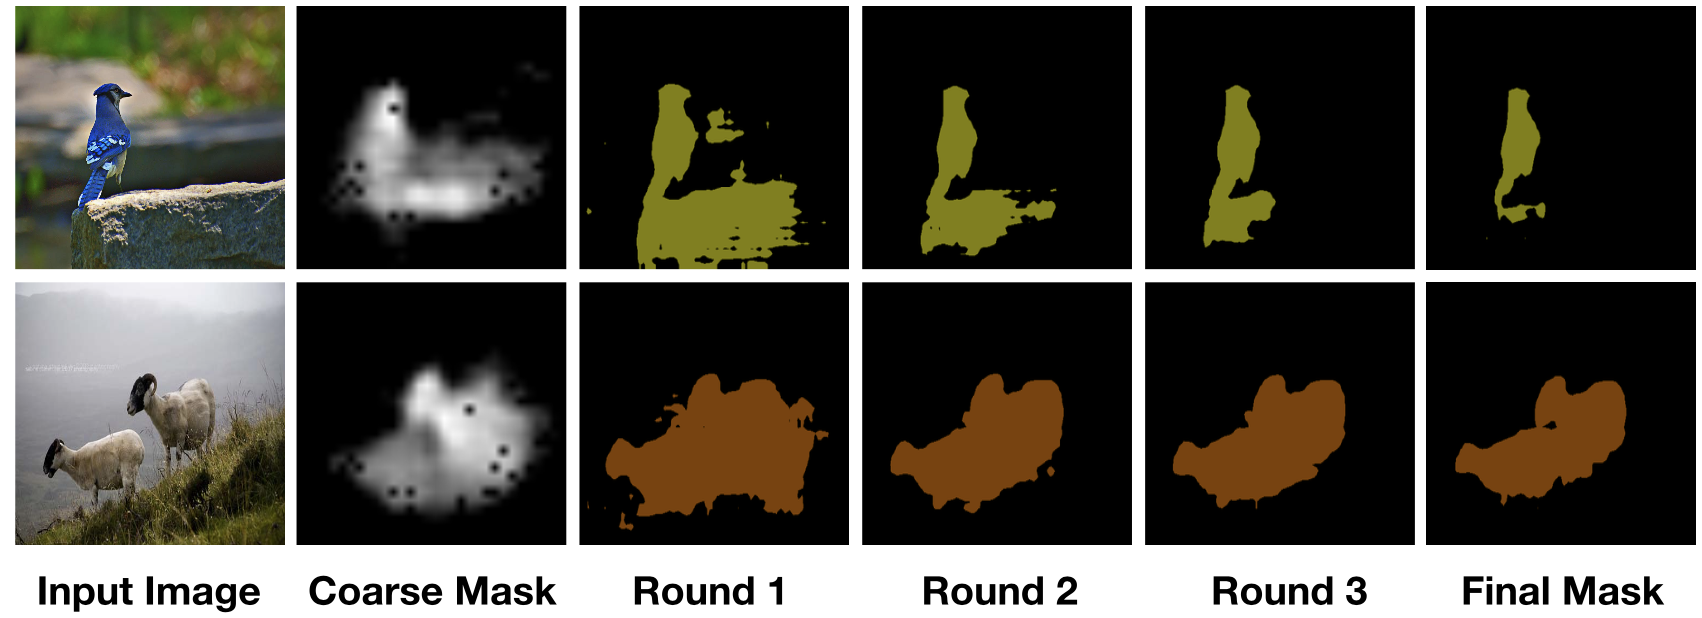
\includegraphics[width = 1 \linewidth]{images/paper6/work.png}
    \centering
    \caption{Example of semantic segmentation generated by the proposed method.}
    \label{fig:semanticWork}
\end{figure}

\subsection{RELATED WORK}
\subsubsection{Semantic Segmentation}
There are three different types of semantic segmentation methods that differ 
based on the level of annotation used:
\begin{enumerate}
    \item \emph{Fully Supervised Pixel-Wise Annotation-Based Methods}: trained with 
    pixel-wise labels annotated by people:
    \item \emph{Weakly Supervised Object-level Annotation-Based-Methods}: trained with 
    methods such as object-level annotations based on the use of bounding 
    boxes;
    \item \emph{Weakly Supervised Image-Level Annotation-Based Methods}: trained 
    with image category labels.
\end{enumerate}
The methods in the first point, if trained with precise labels, are able to 
obtain the best performances.

\subsubsection{Foreground Segmentation}
The labels assigned to pixels can be useful to separate a foreground object 
from a background object. Also for this task there are three strategies to 
perform a segmentation of the objects in the foreground:
\begin{enumerate}
    \item \emph{Joint segmentation-based Methods}: used prior knowledge as supervision.
    \item \emph{Saliency prediction-based Methods}: identify regions present in the human 
    visual scene.
    \item \emph{Object proposal-based Methods}: locate all objects in images.
\end{enumerate}
The proposed framework can also be used for this purpose.

\subsection{THE PROPOSED APPROACH}
\subsubsection{Overview}
The work performed by the model is divided into three steps: \emph{coarse mask 
generation}, \emph{coarse mask enhancement}, and \emph{Recursive mask refinement} (Fig. \ref{fig:step}). In 
order to generate the initial masks, a CNN is trained and subsequently these 
are improved with a graph-based model. Images, enhanced masks and lables 
are used to train the model.
\begin{figure}[h!]
    \centering
    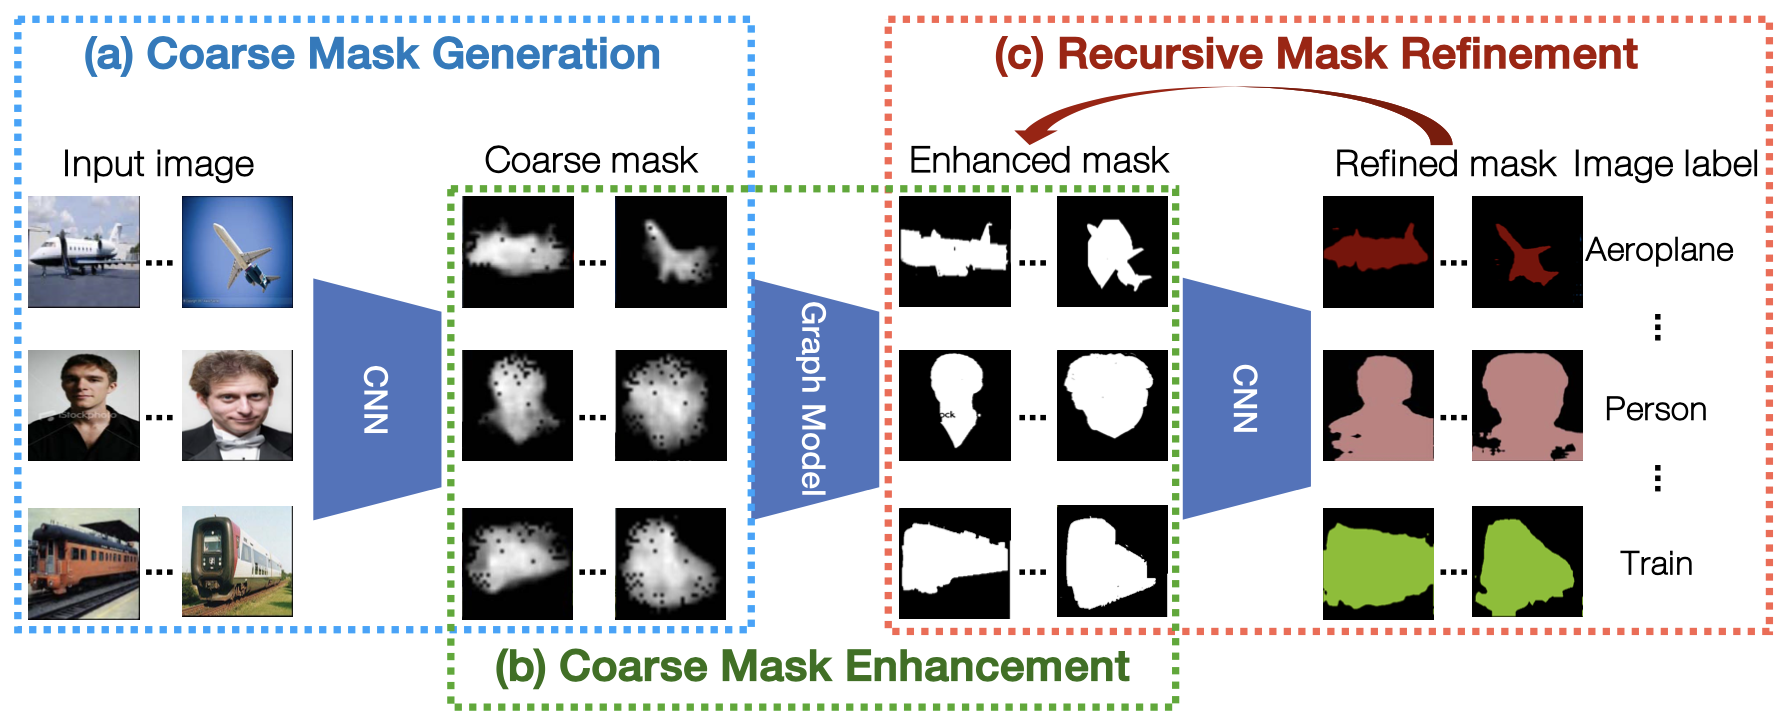
\includegraphics[width = 1 \linewidth]{images/paper6/step.png}
    \centering
    \caption{Steps of the proposed method.}
    \label{fig:step}
\end{figure}

\subsubsection{Coarse Mask Generation}
The generation of a mask must occur without any information on the labels.
The CNN present in \cite{0876055520} is used for this purpose. This network is trained 
with millions of unlabeled images and is also the fastest of other methods 
existing in the state of the art. Unfortunately, as seen in image \ref{fig:semanticWork}, the 
generated coarse masks appear to be inaccurate and do not correspond with 
the position of the underlying object.

\subsubsection{Coarse Mask Enhancement}
The enhancement of the mask is done before the net training process takes 
place. To carry out the improvement, the unsupervised GrubCut model \cite{0876055542} 
is used. This method performs segmentations that divide the background 
from the foreground using a Gaussian Mixture model to estimate the color 
distribution of objects. These distributions are used to construct a Markov 
Random Field on the labels of each pixel. A graph cut optimization has the 
task of maximizing the search for connected regions having the same label. 
There are two steps to apply the GrabCut:
\begin{enumerate}
    \item search for the smallest bounding box inside the mask.
    \item enhance the mask based on the previously created bounding box and on the RGB image.
\end{enumerate}
The enhanced mask will be used to recursively train the network.

\subsubsection{Recursive Mask Refinement}
By combining the labels with the enhanced masks, a semantic segmentation 
is obtained. The purpose is to assign the category label that describes the 
content to the pixels belonging to the foreground. As a semantic segmentation 
network it was decided to use the one called \emph{DeepLab} \cite{0876055502}. This network 
is trained with the improved masks and has the purpose of generating more and more 
precise masks, without noise, which will be used as a new training 
set. Enhancing the mask is a recursive process that will end when the system 
converges to the best representation of the mask. The masks are then used 
as semantic labels to continue training the network.
\begin{figure}[h!]
    \centering
    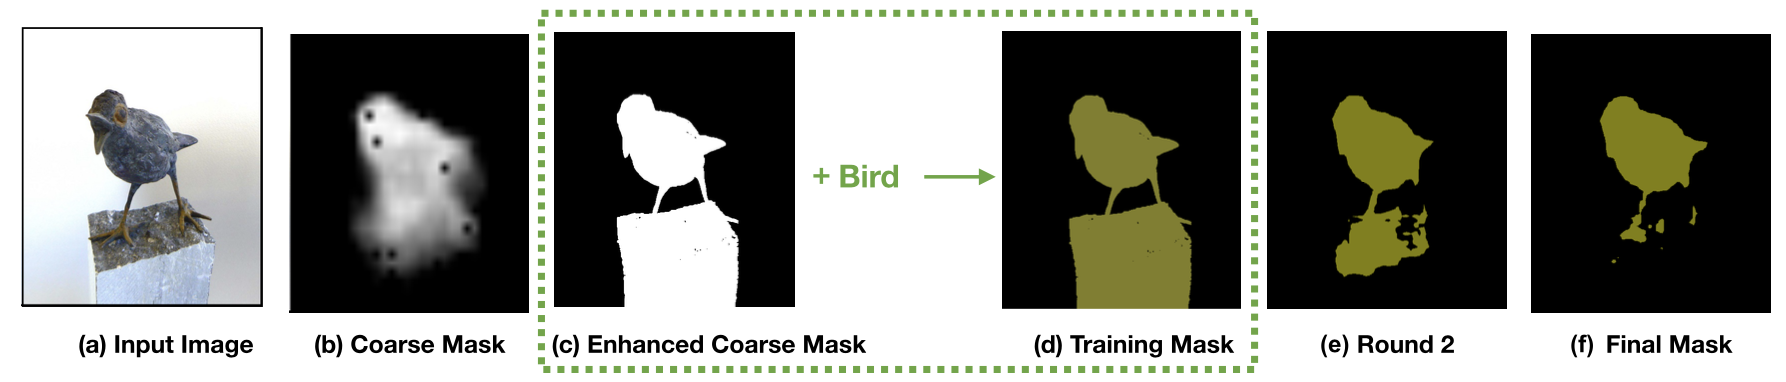
\includegraphics[width = 1 \linewidth]{images/paper6/DeepLab.png}
    \centering
    \caption{The process of semantic mask generation.}
    \label{fig:semanticWork}
\end{figure}

\subsubsection{Model Parameterization}
In summary, to generate high-quality semantic segmentation masks, it is 
required to take an image from the ImgNet dataset and submit it to the 
following steps:
\begin{enumerate}
    \item Create a first mask ($ mask_c $) with a non-superivisoned network \cite{0876055520};
    \item Improve maskc with the GrabCut model \cite{0876055542} to generate a new mask ($ mask_e $);
    \item Train DeepLab network \cite{0876055502} with $ mask_e $;
    \item Generate a better mask ($ mask_r $) using the original ImgNet image;
    \item Enhance the generated mask ($ mask_e $) by applying the GrubCut method;
    \item Repeat from step 3 until the best mask will be obtained.
\end{enumerate}

\subsubsection{Extended the Proposed Framework to Foreground Segmentation}
In order to use the proposed framework in a foreground object recognition 
problem, only the part concerning the enhanced of the mask must be replaced 
with a code that allows to perform the required task. With an architecture 
similar to \emph{FPN} \cite{0876055543}, the new network is called the \emph{Dilated Feature Pyramid 
Network} (DFPN). This network has several dilated layers, in three branches, 
added to enlarge the receptive field of the network (Fig \ref{fig:DFPN}). The features generated 
by these layers are aggregated to make a prediction.
\begin{figure}[h!]
    \centering
    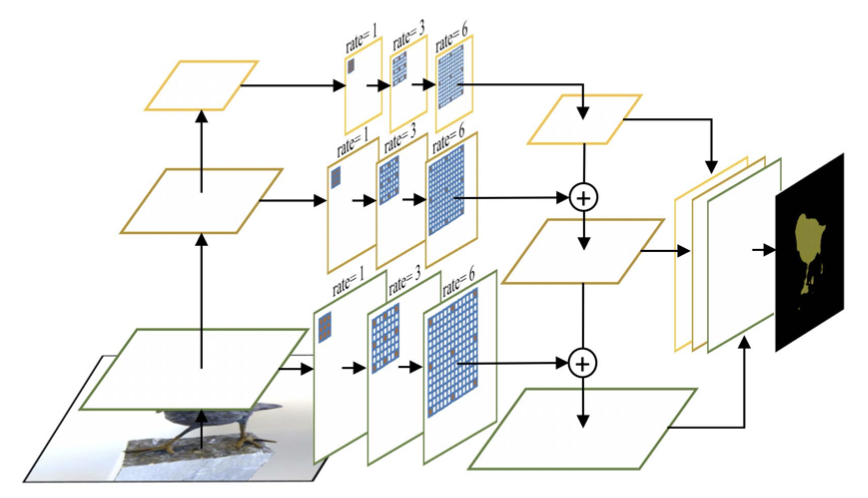
\includegraphics[width = 0.8 \linewidth]{images/paper6/DFPN.png}
    \centering
    \caption{DFPN architecture.}
    \label{fig:DFPN}
\end{figure}

\subsection{EXPERIMENTS}
The network is trained with the images and labels present in ImageNet, while 
the evaluation of the model is carried out on the PASCAL VOC dataset.
\subsubsection{Datasets}
\begin{enumerate}
    \item \emph{ImageNet}: contains about 100,000 labels (synset) annotated by the 
    human, and each label has at least 1000 related images. Two datasets 
    useful for training are formed by ImageNet, these are ImageNet-Sub1 
    and ImageNet-Sub2. The first has a collection of images collected based 
    on the selected category while the second contains images with categories 
    that are not present in the VOC dataset that are present in 
    ImageNet-Sub1.
    \item \emph{VOC}: dataset containing 21 object categories including background. 
    The collection is divided into 3 parts: training, validation and test. In 
    order to be able to evaluate the mask, the results must be sent to the 
    PASCAL VOC evaluation server. 20 image categories are chosen that 
    approximate those of ImageNet as the training dataset.
    \item \emph{MIT Object Discovery Dataset}: this dataset is useful for comparing the 
    results obtained from segmenting objects in the foreground. There are 
    at least three categories of objects in the collection.
\end{enumerate}

\subsubsection{Training Details for Recursive Mask Refinement}
The Stochastic Gradient Descent mini-batch with a batch size of 12 images 
is chosen among the parameters. Parameters such as learning rate, momentum 
and Weight decay are set ad hoc. The training process consists of 5 
rounds where for each of them the mask is continuously improved. The data 
augumentation process is present in every training session.

\subsubsection{Evaluation Metrics}
The \emph{Intersection over Union} (IoU) averaged over 21 categories is used as an 
evaluation index of the semantic segmentation and foreground segmentation. 
This metric is particularly useful for evaluating the accuracy of the identification 
of an object. Both the predicted mask and the ground truth mask 
are required for its calculation. The IoU index is therefore calculated from 
the ratio between the area of overlap and the area of union of the two masks. 
Obviously, the higher this index is, the better the predicted mask will be.

\subsubsection{Semantic Segmentation Results}
\begin{enumerate}
    \item \emph{Impact of the mask quality}: as shown in Table \ref{IoU}, the various processing 
    steps lead to a constant increase in the IoU index. In particular, 
    the value reached by the index is that relating to the first round of 
    network training, therefore we proceed recursively with the training of 
    the network so that it can produce a better mask.
    \begin{table}[h!]
        \centering
        \begin{adjustbox}{max width=\textwidth}
        \begin{tabular}{|c|c|}
            \hline
            Training Mask Type & IoU(\%)\\
            \hline
            Coarse Masks & 32.5 \\
            Bounding Boxes & 35.2 \\
            Enhanced Masks & 47.7 \\
            Refined Masks & 50.4 \\
            \hline
        \end{tabular}
        \end{adjustbox}
        \caption{The performance of semantic segmentation networks evalueted in the validation split of PASCAL VOC dataset in the mean IoU.}
        \label{IoU}
    \end{table}
    
    \item \emph{Effectiveness of recursive refinement}: the evaluation of each refined 
    mask takes place using two types of masks, with or without application 
    of the GrabCut. Between two rounds the masks are improved 
    with a post-processing process by three strategies: a) If the pixels in 
    the foreground are less than 1\% and greater than 80\%, then this image 
    will be discarded by the next training round. b) All the pixels 
    of the original image, labeled with a category must correspond to the 
    predicted pixels with the same category, otherwise these will be considered 
    as background pixels. c) In recursive training, the GrubCut 
    method is applied to the masks that the DeepLab model predicted to 
    have improved masks. In figure \ref{fig:GrubCutApp} it can be seen that the application 
    of GrubCut increases the IoU value and also the system saturates after 
    5 training rounds.
    \begin{figure}[h!]
        \centering
        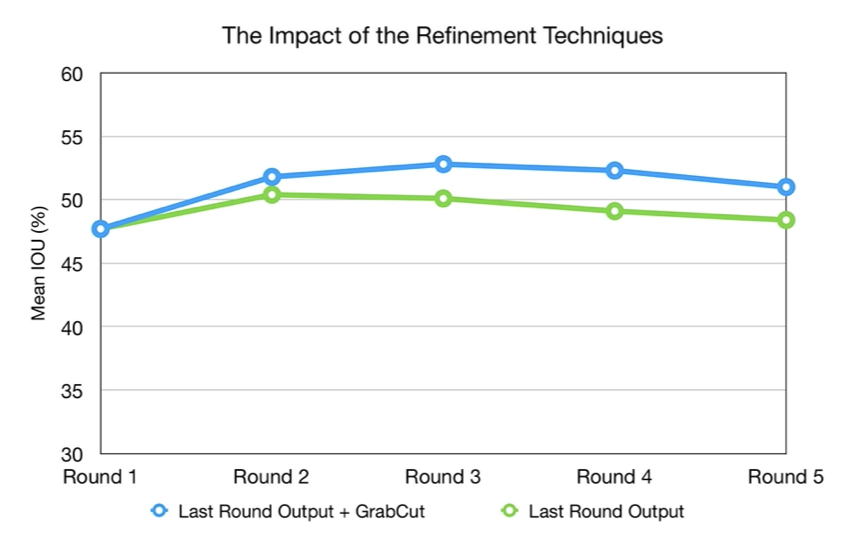
\includegraphics[width = 0.8 \linewidth]{images/paper6/GrabCut.png}
        \centering
        \caption{Enhancement with GrubCut application}
        \label{fig:GrubCutApp}
    \end{figure}

    \item \emph{Comparison with others}: The performance comparison is carried out on both the validation and test sets of the PASCAL VOC dataset (Tab. \ref{IoU score comparison}). In the state of the art, models trained with methods based on object-level labels annotation obtain a better score (greater than 60\%) than models trained with methods that have an annotation of the type image-level labels. The proposed model, on the other hand, while using the image-level labels annotation method, achieves an average IoU score greater than 60\% on both the evaluation and test sets. However, there are several classes in which the model obtains a low IoU value (Fig. \ref{fig:classes}).
    \begin{table}[h!]
        \centering
        \begin{adjustbox}{max width=0.8\textwidth}
        \begin{tabular}{|c|c|c|}
            \hline
            Methods & mIoU(val) & mIoU(test)\\
            \hline
            Supervision: Object-level Labels & &\\
            SDI \cite{0876055513} & 65.7 & 67.5\\
            \hline
            Supervision: Image-level Labels & &\\
            Bootstrap \cite{0876055555} & 63.0 & 63.9\\
            \bfseries{The proposed weakly supervised method} & \bfseries{61.9} & \bfseries{62.8}\\
            \hline
        \end{tabular}
        \end{adjustbox}
        \caption{Comparison, in terms of IoU score, between different models.}
        \label{IoU score comparison}
    \end{table}
    \begin{figure}[h!]
        \centering
        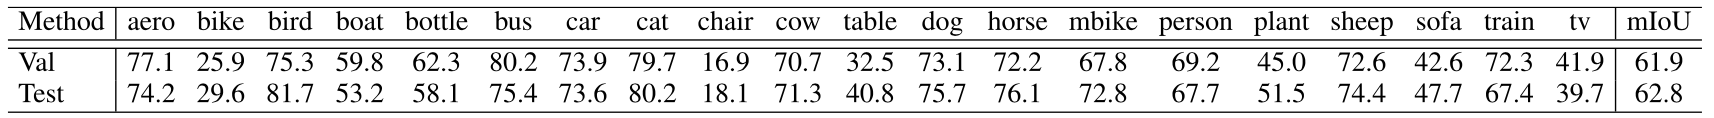
\includegraphics[width = 1 \linewidth]{images/paper6/classes.png}
        \centering
        \caption{Score of IoU in some classes.}
        \label{fig:classes}
    \end{figure}
\end{enumerate}

\subsubsection{Qualitative Results}
Another purpose of the model was to carry out a semantic segmentation also 
on the different objects, belonging to different categories, present in a single 
image, in order to be able to distinguish them. A small example of multiple 
segmentation on different objects is shown in figure \ref{fig:segmentationCategories}.
\begin{figure}[h!]
    \centering
    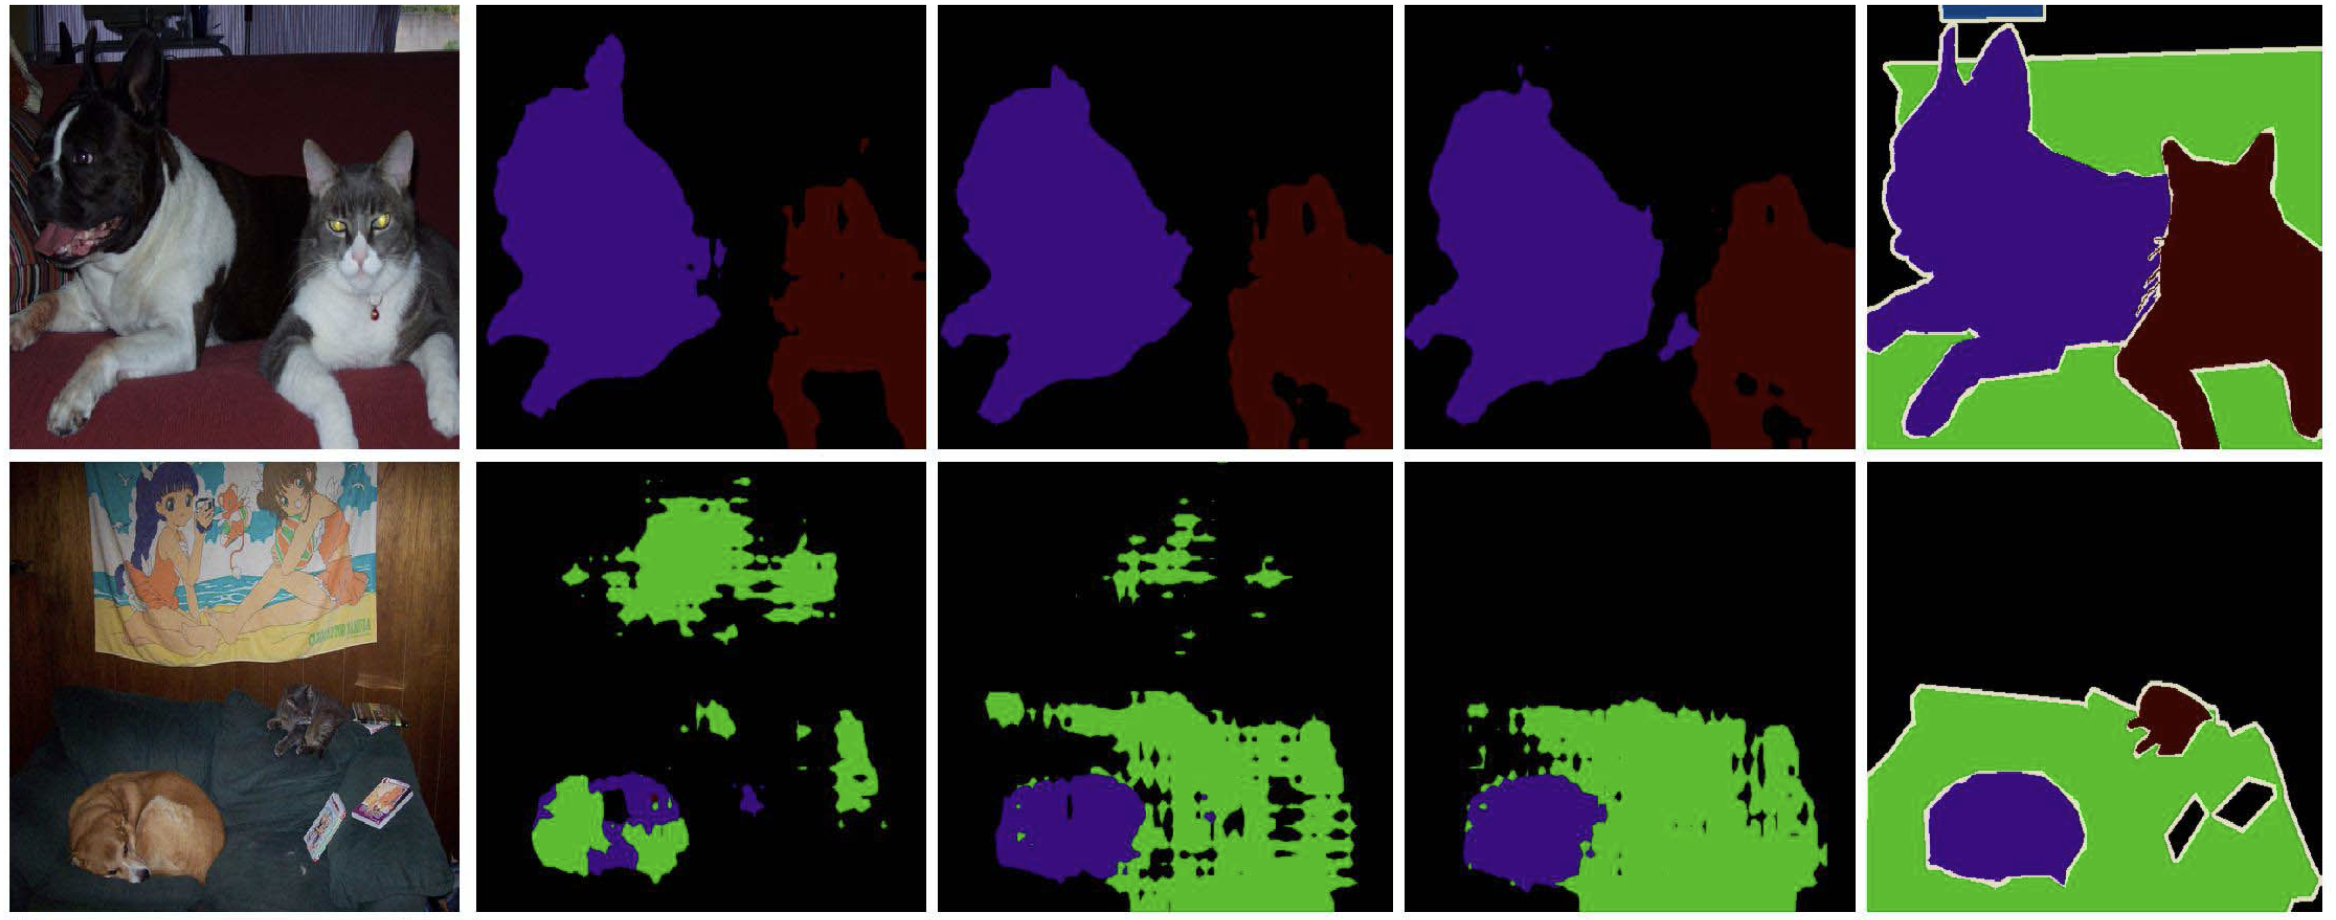
\includegraphics[width = 1 \linewidth]{images/paper6/multiple segmentation.png}
    \centering
    \caption{Example of semantic segmentation on different categories.}
    \label{fig:segmentationCategories}
\end{figure}

\subsubsection{Foreground Segmentations Results}
Also for the segmentation of objects in the foreground, comparisons were 
made with existing models of the state of the art. The dataset used this 
time is that of the MIT Object Discovery unlike the PASCAL VOC used 
in the previous comparisons. From the performance obtained, the proposed 
model, which is remembered to be weakly supervised, manages to achieve the 
performance of the supervised models, with a difference of 2.06\% compared 
to the supervised \emph{PixelObjectness} model \cite{0876055538}.
\begin{table}[h!]
    \centering
    \begin{adjustbox}{max width=\textwidth}
    \begin{tabular}{|c||c|c|c|c||c|c|c|c|}
        \hline
        \multirow{2}{*}{\bfseries{Methods}} & \multicolumn{4}{c||}{\bfseries{MIT dataset (subset)}} & \multicolumn{4}{c|}{\bfseries{MIT dataset (full)}} \\            & \bfseries{Ariplane} & \bfseries{Car} & \bfseries{Horse}  & \bfseries{Average} & \bfseries{Ariplane} & \bfseries{Car} & \bfseries{Horse}  & \bfseries{Average} \\
        \hline
        \bfseries{\#Images} & 82 & 89 & 93 & N/A & 470 & 1208 & 810 & N/A\\
        \hline
        UnsupervisedSeg \cite{0876055520} & 61.37 & 70.52 & 55.09 &62.32 & N/A & N/A & N/A & N/A\\
        \hline
        PixelObjectness \cite{0876055538} & 66.43 & 85.07 & 60.85 &70.78 & 66.18 & 84.80 & 64.90 & 71.96\\
        \hline 
        \bfseries{FPN-Baseline} & 61.09 & 76.22 & 57.89 & \bfseries{65.08} & 61.93 & 75.94 & 64.03 & \bfseries{67.3}\\
        \hline
        \bfseries{Proposed Method} & 64.92 & 77.60 & 60.36 & \bfseries{67.63(+2.57)} & 65.88 & 77.07 & 65.82 & \bfseries{69.59(+2.29)}\\
        \hline
    \end{tabular}
    \end{adjustbox}
    \caption{Quantitative Results of Foreground Segmentation on MIT object Discovery Dataset.}
    \label{}
\end{table}

\subsection{CONCLUSION}
The proposed framework is therefore useful for carrying out a semantic segmentation 
starting with the mask, identified by an unsupervised network for 
the identification of objects in the foreground \cite{0876055520}, and then improving it 
with a fully convolution neural network. The final mask is obtained simply 
by training the model with the annotated labels for each category. The 
method also manages to detect multiple masks for each type of category 
present in each image. It is also possible to identify a foreground object, 
achieving performance equivalent to that of supervised methods.